\section{总体事实}
\subsection{3.1 研究投入}
\begin{frame}{先算每户的研究比率，再跨家庭汇总}
  \strap{3.1\quad 如何定义“每次交易的研究分钟”}
  \[
    r_i=\frac{\text{家庭 }i\text{ 的研究分钟}}{\text{家庭 }i\text{ 的交易次数}}
    \quad\xrightarrow{\text{每户一个比率}}\quad
    \text{家庭间均值与中位数}
  \]
  \begin{tabularx}{\linewidth}{@{}L{.29\linewidth}Y@{}}
    \toprule
    \textbf{分子口径} & \textbf{样本与用途}\\
    \midrule
    宽口径全部研究 & 484户，用于刻画总体投入。包含有交易与无交易的标的。\\
    已交易股票研究 & 50户高股票匹配率样本，只保留归到已交易股票的研究时间。\\
    \bottomrule
  \end{tabularx}
  \finding{登录、查持仓和操作订单的时间另计。分母用该家庭的交易数。}
  \refnote{论文 pp.~12、15–21，Table 2。}
\end{frame}

\begin{frame}{为什么144.2分钟和5.7分钟同时成立？}
  \strap{3.1\quad 比较顺序：同一组横读，再比较同一50户的两种分子}
  \centering
  \begin{tikzpicture}[x=.043cm,y=1cm]
    \foreach \x in {0,30,60,90,120,150}{
      \draw[quiet!18] (\x,0)--(\x,3.54);
      \node[below,font=\scriptsize] at (\x,0) {\x};
    }
    \foreach \y/\k/\m/\d/\sty in {3.12/{484户 · 宽口径}/144.2/36.4/ink,
      2.02/{50户 · 宽口径}/96.8/51.7/ink,
      .92/{同一50户 · 已交易股}/29.1/5.7/wine}{
      \node[anchor=east,font=\small,text=\sty] at (-3,\y) {\k};
      \fill[slate] (0,\y+.02) rectangle (\m,\y+.25);
      \fill[wine] (0,\y-.29) rectangle (\d,\y-.06);
      \node[anchor=west,font=\small\bfseries,text=slate] at (\m,\y+.135) {\m};
      \node[anchor=west,font=\small\bfseries,text=wine] at (\d,\y-.175) {\d};
    }
    \node[anchor=east,font=\scriptsize] at (150,-.55) {分钟／交易};
    \node[anchor=west,font=\scriptsize] at (0,-.55) {\textcolor{slate}{\rule{8pt}{5pt}}\ 均值
       \quad \textcolor{wine}{\rule{8pt}{5pt}}\ 中位数};
  \end{tikzpicture}
  \raggedright
  \finding{均值受高投入家庭影响。在同一50户里，分子限于已交易股时，中位数为5.7。}
  \refnote{按 Table 2 Panels B–C（p.~47）重绘。先户内归一，再跨家庭汇总。}
\end{frame}

\subsection{3.2 研究渠道}
\begin{frame}{券商站外占了均值研究时间的一半以上}
  \strap{3.2\quad 跨站覆盖为何会改变所见的投入}
  \vspace{2mm}
  \begin{center}
    \begin{tikzpicture}[x=.068cm,y=1cm]
      \fill[slate] (0,0) rectangle (55.7,.88);
      \fill[wine] (55.7,0) rectangle (101,.88);
      \fill[wine!82!black] (101,0) rectangle (142.9,.88);
      \fill[quiet!65] (142.9,0) rectangle (144.2,.88);
      \node[white,align=center,font=\small] at (27.85,.44) {券商\\55.7};
      \node[white,align=center,font=\small] at (78.35,.44) {Yahoo Finance\\45.3};
      \node[white,align=center,font=\small] at (121.95,.44) {其他财经\\41.9};
      \draw[quiet] (143.55,.9)--(143.55,1.25)--(123,1.25);
      \node[anchor=east,font=\scriptsize] at (123,1.25) {公司网站 1.3};
      \node[anchor=west,font=\small,text=quiet] at (0,-.42) {484户，家庭比率的均值，分钟／交易};
    \end{tikzpicture}
  \end{center}
  \medskip
  \nextq{渠道告诉我们研究发生在哪里。接下来分辨打开的是什么内容。}
  \refnote{Table 2 Panel B（p.~47），论文 pp.~16–19。站外份额按均值分钟计算。}
\end{frame}

\subsection{3.3 内容与窗口}
\begin{frame}{价格图既覆盖广，也占用较多研究时间}
  \strap{3.3\quad 同时看参与比例和分钟，区分广度与投入}
  \begin{tabularx}{\linewidth}{@{}Yrr@{}}
    \toprule
    \textbf{直接分类} & \textbf{参与家庭比例} & \textbf{均值分钟／交易}\\
    \midrule
    \textcolor{wine}{\textbf{价格图}} & \textcolor{wine}{93\%} & \textcolor{wine}{39.1}\\
    综合行情 & 93\% & 37.0\\
    分析师资料 & 71\% & 12.5\\
    其他基本面 & 53\% & 2.6\\
    盈利 & 40\% & 1.7\\
    \textcolor{slate}{传统风险统计} & 约1\%（7户） & 0.0（四舍五入）\\
    \bottomrule
  \end{tabularx}
  \finding{少有家庭专门查询标准风险统计。行情与价格图仍可能提供波动线索。}
  \refnote{Table 3 左侧直接分类（p.~48），p.~24。484户，宽口径。}
\end{frame}

\begin{frame}{综合行情同时展示多种信息}
  \strap{3.3\quad 从“看了哪种页面”到“可能接触了什么内容”}
  \begin{columns}[T,onlytextwidth]
    \column{.47\textwidth}
      \begin{tikzpicture}
        \node[storyfocus,text width=4.8cm,minimum height=2.4cm] (s)
          {\textbf{综合行情}\par\medskip
           即时报价 \quad 价格图\par
           盈利指标 \quad 分红信息};
      \end{tikzpicture}
      \par{\scriptsize 页面结构示意}
    \column{.49\textwidth}
      \shortlabel{价格图的均值分钟／交易}\par
      \greatnum{39.1}\ \ $\longrightarrow$\ \ \greatnum{64.4}\par
      {\small\hspace{1mm}直接分类\hspace{10mm}分配混合内容后}
  \end{columns}
  \medskip
  \finding{三类混合页面约占均值总量42\%。归因调整各主题份额，总分钟保持不变。}
  \refnote{Table 3、附录 Table IA2。三类为综合行情、内容不明新闻和讨论板。约42\%为据表计算。}
\end{frame}

\begin{frame}{含默认展示时，实际看到的多是日内图}
  \strap{3.3\quad 先看接触到的历史长度}
  \begin{columns}[c,onlytextwidth]
    \column{.70\textwidth}
      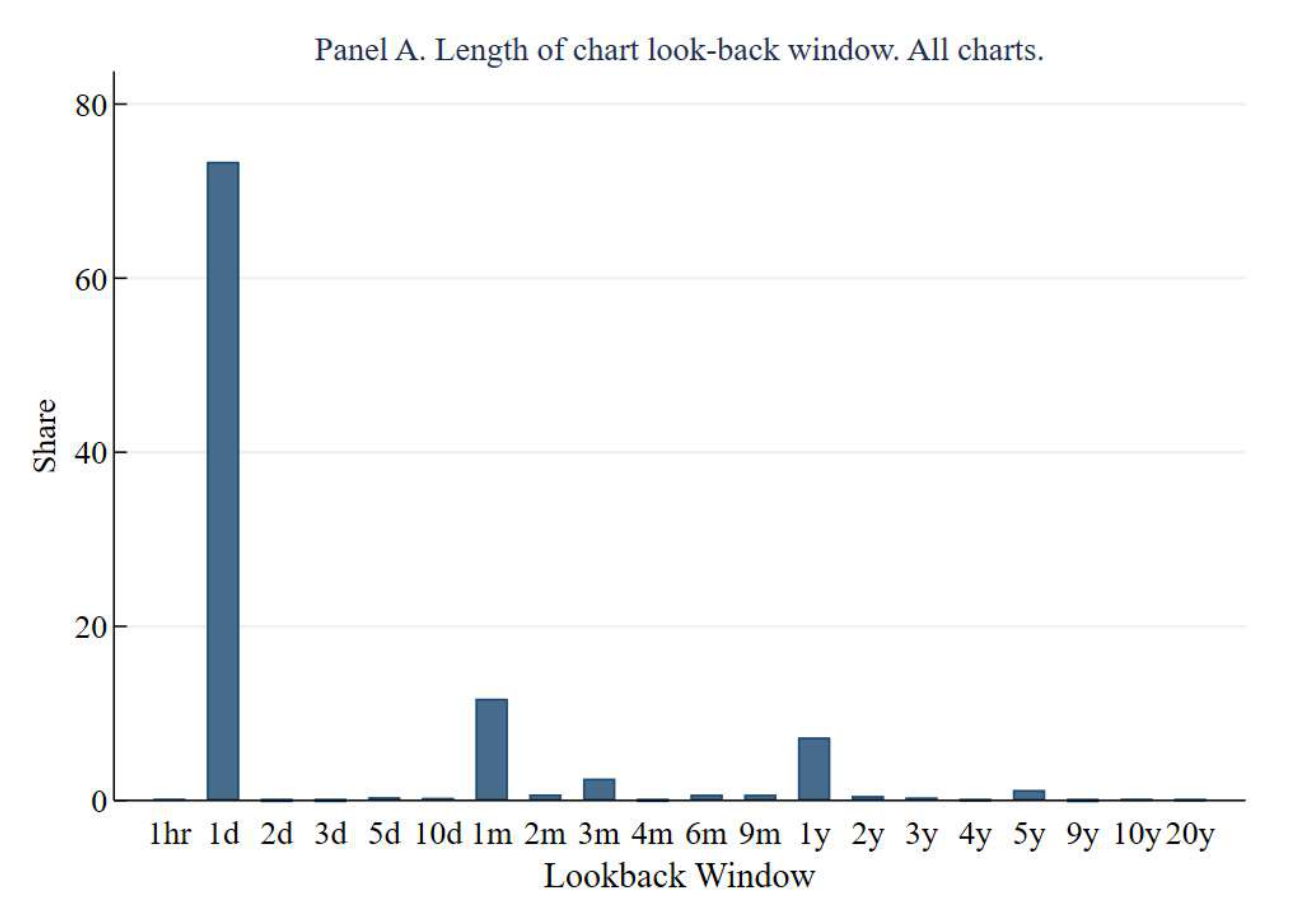
\includegraphics[width=\linewidth,height=4.72cm,keepaspectratio]{lookback-all.png}
    \column{.27\textwidth}
      \greatnum{\(>70\%\)}\par
      {\small 图表属于日内窗口}\par
      \medskip
      {\small 先定位横轴 \textbf{1d}，再读该柱在面板内的份额。}
  \end{columns}
  \refnote{Figure 1A（p.~52），p.~27。全样本，图表包含默认显示。}
\end{frame}

\begin{frame}{主动调整窗口时，常选择更长的历史}
  \strap{3.3\quad 再看主动调整者的选择}
  \begin{columns}[c,onlytextwidth]
    \column{.70\textwidth}
      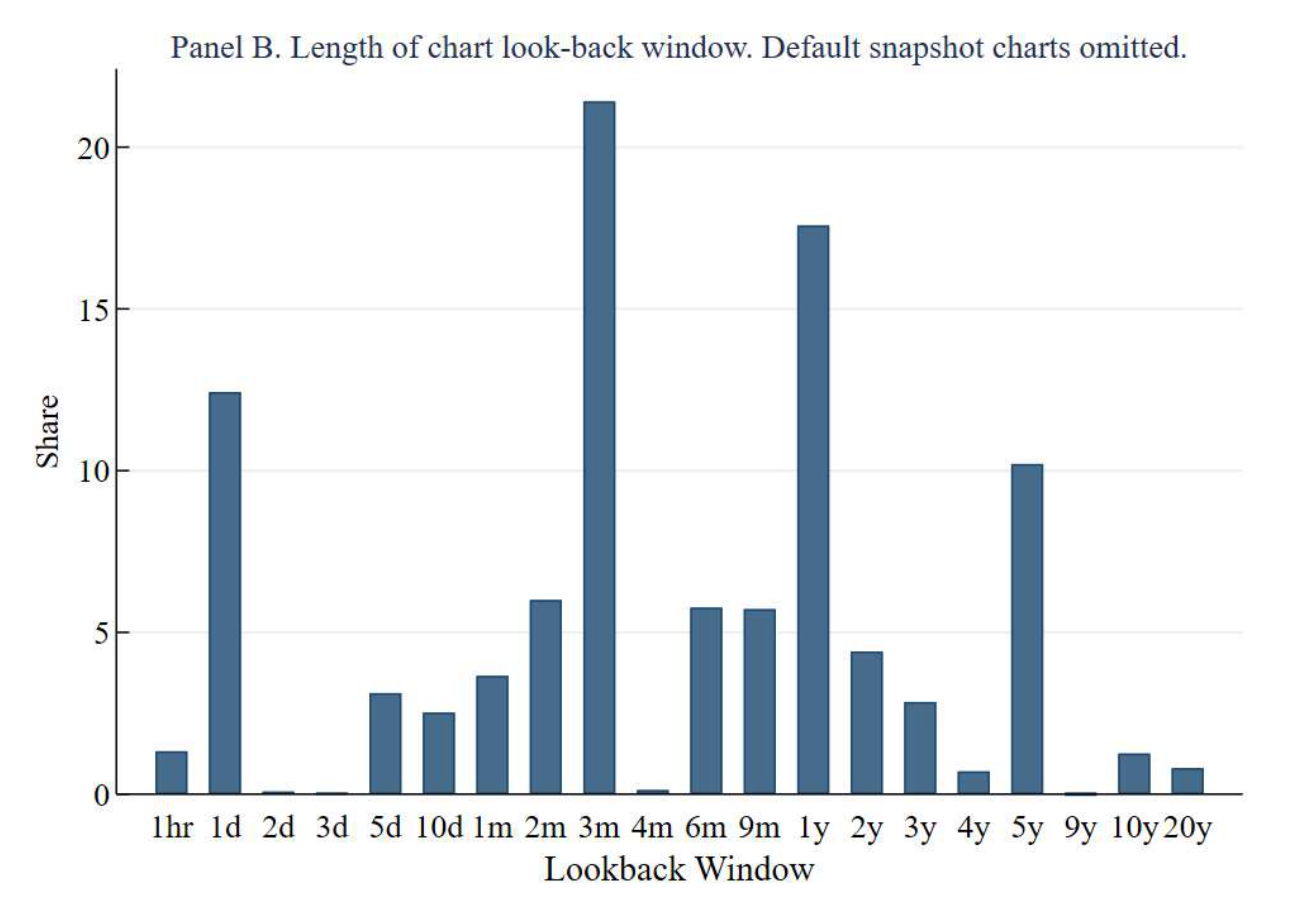
\includegraphics[width=\linewidth,height=4.72cm,keepaspectratio]{lookback-opt-in.png}
    \column{.27\textwidth}
      \textcolor{wine}{\bfseries 一个月至一年}\par
      \medskip
      {\small 先看3m和1y。两面板的分母与纵轴尺度有别。}
  \end{columns}
  \nextq{总体内容画像由哪些股票和家庭形成？}
  \refnote{Figure 1B（p.~52），p.~27。面板描述主动选择的窗口，按原图裁剪。}
\end{frame}
